\documentclass[handout]{beamer}
\usepackage{beamerthemesplit}
\usepackage{pgfpages}
\usepackage{verbatim}
\usepackage{amsmath, amssymb, graphics, setspace}

\usepackage{algorithm}
\usepackage{algorithmicx}
\usepackage{algpseudocode}


\newcommand{\field}[1]{\mathbb{#1}} %requires amsfonts

\usetheme{Antibes}
\usecolortheme{beaver}
\title[Thesis Progress Report \#5]{Thesis Progress Report \#5}

\usepackage{mathptmx}
\usepackage[scaled=.90]{helvet}
\usepackage{courier}
\usepackage[T1]{fontenc}

%\pgfpagesuselayout{4 on 1}[letterpaper,border shrink=5mm]

\institute[RIT]{}
\date{\today}
%\subtitle{}
\author{Christopher A. Wood}
%\institute[]{}
\date{\today}

\begin{document}

%%%%%
%%
%% Resource link: http://www.math-linux.com/spip.php?article77
%%
%%%%

\begin{frame}
	\titlepage
\end{frame}

\begin{frame}
	\frametitle{Agenda}
	\tableofcontents
\end{frame}

\section{Revisiting last week's questions}
\begin{frame}
	\frametitle{Questions Answered}
	How many irreducible and primitive polynomials exist for extension fields $GF((2^n)^m)$?
	\begin{itemize}
		\item $(n,m) = (2,2) = 18$
		\item $(n,m) = (2,3) = 180$
		\item $(n,m) = (3,2) = 504$
		\item $(n,m) = (2,4) = 1800$
		\item $(n,m) = (4,2) = 10800$
		\item ...
	\end{itemize}
\end{frame}

\section{Algebraic Complexity of AES-like S-boxes}
\begin{frame}
	\frametitle{Determining the algebraic complexity}
	\begin{itemize}
		\item The AES S-box is a function $S(x) = L(x) \oplus b$, where $L(x)$ is a linear
		function over $GF(2)$.
		\item There are many ways to represent $S(x)$ as a polynomial equation:
		\begin{itemize}
			\item Lagrangian interpolation
			\item Polynomial linearization
			\item q-ary polynomial deduction
		\end{itemize}
	\end{itemize}
\end{frame}

\begin{frame}
	\frametitle{Lagrangian Interpolation}
	For any function $F : \mathbb{Z}_n \to \mathbb{Z}_n$ with input $x_1,\dots,x_n$ and output $y_1,\dots,y_n$, we may 
	find a polynomial representation $P(x)$ as follows: 
	\begin{align*}
P(x) = \sum_{i = 0}^{k-1}P_i(x),
	\end{align*}
	where
	\begin{align*}
P_i(x) = y_i \prod_{j=1, j\not=i}^{k} \frac{x - x_j}{x_i - x_j}
	\end{align*}
\end{frame}

\begin{frame}
	\frametitle{A Simple Example}
	Let $F : GF(2^2) \to GF(2^2)$ be a function defined in $GF(2^2)/p(x) = x^2 + x + 1$ by the following map:
	\begin{align*}
		0 & \to 1 \\
		1 & \to \alpha \\ 
		\alpha & \to \alpha + 1\\
		\alpha + 1 & \to 0
	\end{align*}
	For Lagrangian interpolation, we need polynomials $f_z(x)$ with the property $f_z(x) = 1$ and $f_z(y) = 0$ if $y \not= z$.
\end{frame}

\begin{frame}
	\frametitle{A Simple Example}
	Start by constructing the polynomial $g(x) = (x - 1)(x - \alpha)(x - (\alpha + 1))$. Note that if $x \in GF(2^2) \setminus \{0\}$, then
	$g(x) = 0$.
	
	\medskip
	
	Therefore, we pick $f_0(x) = g(x) / g(0)$, where $g(0) = 1 \cdot \alpha \cdot (\alpha + 1) = 1$
	
	\medskip
	
	Thus, $f_0(x) = g(x)$, which makes this very easy. Expanding out $g(x)$ yields:
	\begin{align*}
		g(x) & = (x-1)(x-\alpha)(x-(\alpha+1)) \\
		& = (x^2 - x - x\alpha + \alpha)(x-(\alpha+1))\\
		& = x^3 - x^2 -x^2\alpha + x\alpha - x^2\alpha - x\alpha - x\alpha^2 -\alpha^2 +x^2 -x -x\alpha + \alpha
		& = x^3 + 1,
	\end{align*}
	after reduction with $p(x) = x^2 + x + 1$, of course.
\end{frame}

\begin{frame}
	\frametitle{A Simple Example}
	We may find the other polynomials $f_1(x), f_{\alpha}(x), f_{\alpha+1}(x)$ by linear substitutions:
	\begin{align*}
		f_z(x) = f_0(x-z)
	\end{align*}
	(A textbook informed me of this fact)
\end{frame}

\begin{frame}
	\frametitle{A Simple Example}
	Now we can do interpolation as follows:
	\begin{align*}
		q(x)& = F(0)f_0(x) + F(1)f_1(x) + F(\alpha)f_{\alpha}(x) + F(\alpha+1)f_{\alpha+1}(x)\\
		& = x^2(\alpha + 1) + 1
	\end{align*}
	
	\medskip
	
	A simple check...
	\begin{align*}
		q(\alpha)  = (\alpha)^2(\alpha + 1) + 1 = \alpha^3 + \alpha^2 + 1 = \alpha + 1\\
		q(1) = (1)^2(\alpha + 1) + 1 = \alpha\\
		q(0) = (0)^2(\alpha + 1) + 1 = 1 \\
		q(\alpha + 1) = (\alpha + 1)^2(\alpha + 1) + 1 = \alpha^3 + \alpha + \alpha^2 = 0 
	\end{align*}
\end{frame}

\begin{frame}
	\frametitle{Lagrangian Lesson}
	The method is more symbolic than computational (at first glance), so perhaps there's a better way
	to estimate the complexity...
\end{frame}

\begin{frame}
	\frametitle{Polynomial Linearization}
	\begin{itemize}
		\item Any linear function $A$ over $GF(2^k)$ can be represented as a matrix multiplication
		\item Similarly, such functions can be represented by a linearized polynomial:
		\begin{align*}
			f(\alpha) = \sum_{i = 0}^{k-1}\lambda_i \alpha^{2^{i}}
		\end{align*}
		\item Solve for $\lambda_i$ by setting up and solving a system of linear equations 
		\begin{itemize}
			\item Select some $\alpha$, compute $A(\alpha)$ and $\alpha^{2^{i}}$ for all $0 \leq i \leq k-1$
			\item Solve for each $\lambda_i$ using Gaussian elimination
		\end{itemize}
	\end{itemize} 
\end{frame}

% \begin{frame}
% 	\frametitle{Polynomial Linearization Continued}
% 	\begin{itemize}
% 		\item Alternatively, solve for $\lambda_i$ using dual basis decomposition
% 		\item Let $A$ be a linear function defined by 
% 		$A(x) = \sum_{i=0}^{k-1} f_i\alpha^i = f_0 + \alpha f_1 + \alpha^2 f_2 + \dotsb + \alpha^{k-1}f_{k-1}$,
% 		where $\{\beta^0,\beta^1,\dots,\beta^{k-1}\}$ is the dual basis for $\alpha$
% 		\item Let $f_i = Tr(g(x)\beta_i)$, where $g(x) = \sum_{i=0}^{k-1}\alpha_i f_i()$
% 	\end{itemize} 
% \end{frame}

\begin{frame}
	\frametitle{Bounds on Algebraic Expression}
	The upper bound on the number of terms in an algebraic expression for affine-power functions 
	\begin{align*}
	F(x) = A(P(x))
	\end{align*}
	in $GF(2^n)$ is $n + 1$
	
	\medskip
	
	The forward AES S-box, $F(X) = L(x^{-1}) = L(x^{254})$, has $9$ terms:
	\begin{align*}
		L(x) = \sum_{i=0}^{7}\lambda_i x^{2^{i}}
	\end{align*}
\end{frame}

\begin{frame}
	\frametitle{Increasing the Algebraic Complexity}
	\begin{itemize}
		\item Affine-power-affine functions: $F(x) = A \circ P \circ A$
		\begin{itemize}
			\item Increases algebraic complexity without affecting other cryptographic properties (strict avalanche, nonlinearity, differential uniformity, algebraic degree)
			\item This increased the algebgraic complexity from 9 to 253
		\end{itemize}
		\item Gray code augmentation: $F(x) = L \circ P \circ G$
		\begin{itemize}
			\item A \emph{gray code} is a binary numeral system where two successive values differ by a single bit
			\item $G$ is gray-code conversion from an element $x \in GF(2^n)$ to a corresponding gray-code
			\item Conversion process: $y_i = x_{i+1} \oplus x_i$ and $y_n = x_n$
		\end{itemize}
		% SIPJACK S-box?
		\item M\"{o}bius transformation: $f(z) = \frac{az + b}{cz + d}$, where $a,b,c,d \in GF(2^k)$.
	\end{itemize}
\end{frame}

\section{Boolean Function Constructions}
\begin{frame}
	\frametitle{General Maiorana-McFarland Construction}
	\begin{itemize}
		\item Concatenate small affine functions to form higher-order functions
		\item (Hopefully) the result is an equally strong Boolean function
		\item All MM Boolean functions have an annihilator of degree $(n - r + 1$), where $r$ is the number of variables of affine functions
		which are used (concatenated) to construct the function
		\item As $r$ decreases the annihilator degree increases, making algebraic attacks easier (it simplifies the equations)
	\end{itemize}
\end{frame}

\begin{frame}
	\frametitle{Linear Codes}
	\begin{itemize}
		\item A $[n,k,d]$-code (binary code) is a subspace of $\mathbb{F}_2^n = GF(2)^n$ 
		\begin{itemize}
			\item $n$ is the length, $k$ is the rank, $d$ is the minimum (Hamming) distance between each codeword in the subspace
		\end{itemize}
		\item The vectors of a binary linear code are called the \emph{codewords}
		\item As a subspace, there exists a basis $\mathbf{B}$ for the code, which is often represented as a \emph{generator matrix} $\mathbf{G}$
		\item Many codes of cryptographic interest: Hamming, Walsh-Hadamard, \dots
	\end{itemize}
\end{frame}

\begin{frame}
	\frametitle{Candidate Codes}
	\begin{itemize}
		\item Hamming Code: a special type of binary $[n,k,3]$ code
		\begin{itemize}
			\item Mainly used for error detection/correction, but we can use it for resilient BF constructions
		\end{itemize}
		\item Hadamard Code: a special type of binary $[2^k, k, 2^{k-1}]$ code
	\end{itemize}
\end{frame}

\begin{frame}
	\frametitle{Construction Idea for $t$-resilient}
	\begin{itemize}
		\item Let $f_1,\dots,f_{2^{n-r}}$ be $2^{n-r}$ affine Boolean functions of length $2^r$ (i.e. the truth table has $2^r$ entries)
		\item Concatenating $f_1,\dots,f_{2^{n-r}}$ yeilds a string of length $2^n$
		\item Let $g(x_n,\dots,x_{r+1})$ be a nonlinear function and let $h(x_r,\dots,x_1)$ be a linear (affine) function, and let $f(x_n,\dots,x_1) = g(x_n,\dots,x_{r+1})\oplus h(x_r,\dots,x_1)$
%		\item 
	\end{itemize}
	*Note: all Boolean functions are $(t+1)$ degenerate, for reasons that are discussed in the paper :-)
\end{frame}

\begin{frame}
	\frametitle{Construction Idea for $t$-resilient}
	\begin{itemize}
		\item Select a $[n = u, k = m, d = t + 1]$ code and construct a $(2^m - 1)\times m$ matrix with codewords from $C$ s.t. 
		$\{ c_1D_{i,1} \oplus \dotsb \oplus c_mD_{i,m} : i \leq 1 \leq 2^m - 1 \} = C \setminus \{\bar{0}\}$. Let $L(C)$ be a
		$(2^m - 1) \times m$ matrix whose entries are $u$-variable functions defined by $L_{i,j}(x_1,\dots,x_u))$
		\item Define an $(p,m)$ S-box with component functions $G_1,\dots,G_m$, and let $L(C,k,l)$ be an $(l-k+1)\times m$ matrix whose
		$i,j$th entry is
		\begin{align*}
			G_j(y_1,\dots,y_p) \oplus L_{k+i-1,j}(x_1,\dots,x_u).
		\end{align*}
	\end{itemize}
\end{frame}

\begin{frame}
	\frametitle{Construction Continued}
	\begin{itemize}
		\item If $l - k + 1 = 2^r$ then $G \oplus L(C,k,l)$ is an $(r+p+u,m)$ S-box: 
		\begin{align*}
			F_j(z_1,\dots,z_r,y_1,\dots,y_p,x_1,\dots,x_u) = \\
			G_j(y_1,\dots,y_p) \oplus L_{k+i-1,j}(x_1,\dots,x_u)
		\end{align*}
		\item Goal: Let $m = 16$, find other parameters that make the construction ``work''
		\item Need to select good $(p,16)$ S-boxes $G_1,\dots,G_m$ and \emph{find} a good $[n,16,t+1]$ code word
	\end{itemize}
\end{frame}

\section{Software Optimizations for S-Box}
\begin{frame}
	\frametitle{Software Optimizations for S-Box}
	\begin{itemize}
		\item Extended Euclidean Algorithm - Straightforward
		\item Binary Extended Euclidean Algorithm - Optimized version of EEA for fields of characteristic 2
		\item Normal basis conversion with Fermat's Theorem - Two matrix multiplications with some shifting and multiplying
		\item Almost Inverse Algorithm - Compute $A^{-1}x^k \mod f(x)$ and then reduce by $x^k$
		\item Bitsliced implementation - Carnright investigates this technique with his normal basis optimizations
		\item LUTs - Not a goal, but always an option...
	\end{itemize}
\end{frame}

\begin{frame}
	\frametitle{Software Optimizations for S-Box - Metrics}
	These can be captured with gprof for different platforms...
	\begin{itemize}
		\item Extended Euclidean Algorithm - TODO		
		\item Binary Extended Euclidean Algorithm - TODO
		\item Normal basis conversion with Fermat's Theorem - TODO
		\item Almost Inverse Algorithm - TODO
		\item Bitsliced implementation - TODO
		\item LUTs - ;-)
	\end{itemize}
\end{frame}

\section{16-Bit Circuit for Multiplicative Inverse Calculation}
\begin{frame}
	\frametitle{Complexity of Finite Field Multipliers}
	\begin{itemize}
		\item Claim: for small fields (e.g. $GF(2^k), k \leq 32$) the \emph{arithmetic} procedures for 
		software implementations \textbf{are not} affected by the field polynomial.
		\begin{itemize}
			\item Advanced algorithms such as the ``comb'' multiplier target fields where
			single elements cannot fit within a single word
		\end{itemize}
		\item This is not true for hardware...
		\begin{itemize}
			\item If we're going for area optimized designs, we want serial modules, otherwise
			we want parallel modules
			\item Some bases yield more efficient arithmetic operations than others
			\item This leads us to Optimal Normal Bases
		\end{itemize}
	\end{itemize}
\end{frame}

\begin{frame}
	\frametitle{Inverse by Fermat's Theorem}
	By Fermat's Theorem, $\alpha^{-1} \equiv \alpha^{2^k - 2}$
	
	\medskip
	
	\begin{align*}
		2^{m-2} = 2 + 2^2 + 2^3 + \dotsb + 2^{m-1}
	\end{align*}
	
	This leads us to a simple square and multiply algorithm...
	
	\begin{align*}
		\alpha^{-1} = \alpha^2 \cdot \alpha^{2^{2}} \cdot \alpha^{2^{3}} \dotsb \cdot \alpha^{2^{m-1}}
	\end{align*}
	
	In a normal basis the cycle complexity is $\mathcal{O}(k)$ for computing the successive powers of $\alpha$, but the 
	area complexity depends on the type of multiplier used (e.g. using a ONB Type II basis one can implement a parallel 
	multiplier with $1.5(k^2 - k)$ XOR gates [1])
\end{frame}

% \begin{frame}
% 	\frametitle{Inverse by Fermat's Theorem (Continued)}
% 	\begin{center}
% 	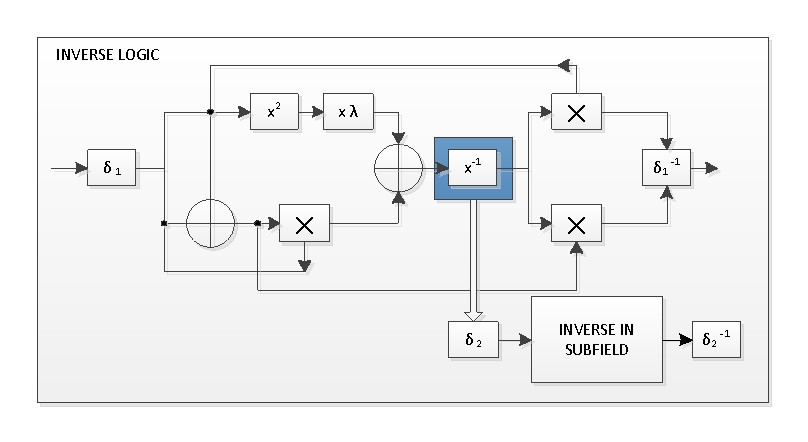
\includegraphics[scale=.35]{./composite_field_inverter.pdf}
% 	\end{center}
% \end{frame}

\begin{frame}
	\frametitle{Inverse by Composite Field Computation}
	$(bx + c)^{-1} = b(b^2B + bcA + c^2)^{-1}x + (c + bA)(b^2B + bcA + c^2)^{-1}$ with $A = 1$ and $B = \lambda$
	\begin{center}
	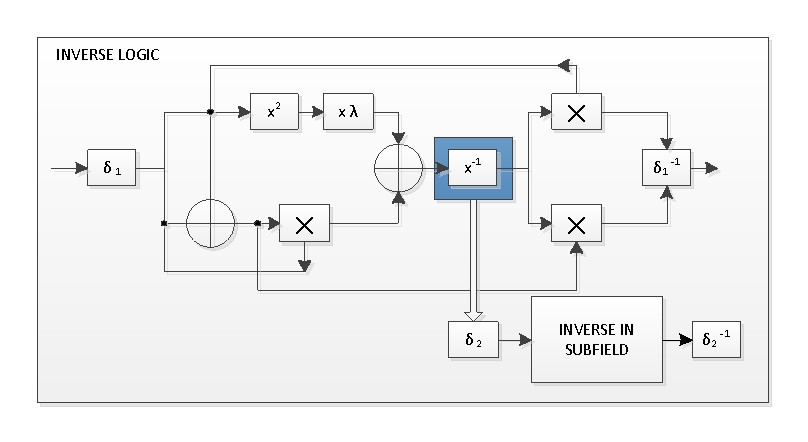
\includegraphics[scale=.7]{./composite_field_inverter.pdf}
	\end{center}
\end{frame}

\begin{frame}
	\frametitle{Inverse by Composite Field Computation (continued)}
	$5$-stage pipeline design
	\begin{center}
	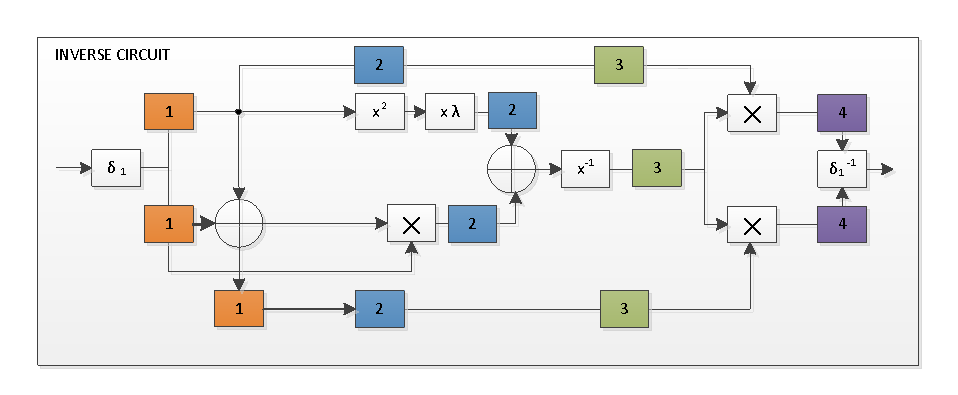
\includegraphics[scale=.7]{./composite_field_inverter_pipeline.pdf}
	\end{center}
\end{frame}

\begin{frame}[fragile]
	\frametitle{Optimal Pipeline Selection Strategy (for FPGAs)}
\begin{algorithm}[H] 
\caption{Pipeline Optimization Strategy} 
\begin{algorithmic}[1]
% \Require{Functionally correct pipeline version of the inverse circuit.}
% \Ensure{An efficient pipeline implementation.}
\State $E_c = Throughput(Mbits/s)/Area$
\State $Opt \gets False$
\While {$Opt = False$}
	\State Remove the pipeline state that contributes the lowest frequency reduction
	\State Reimplement and resynthesize the design
	\State $E_n = Throughput(Mbits/s)/Area$
	\If{$E_c > E_n$}
		\State $Opt = True$
	\EndIf
\EndWhile
\end{algorithmic}
\end{algorithm}
\end{frame}

\begin{frame}
	\frametitle{Inverse by Composite Field Computation (continued)}
	The next step is to synthesize the design and gather hardware metrics. 
	\begin{itemize}
		\item LUT count (FPGA - captured with Xilinx tools)
		\item Register count (FPGA - captured with Xilinx tools)
		\item Slice count (FPGA - captured with Xilinx tools)
		\item Throughput in cycles/byte (FPGA - captured with Xilinx tools)
		\item Power consumption (ASIC - captured with Synopsys) :-)
	\end{itemize}
\end{frame}

% \begin{frame}
% 	\frametitle{Tasks}
% 	\begin{itemize}
% 		\item 
% 		\item 
% 		\item 
% 	\end{itemize}
% \end{frame}

% \begin{frame}
% 	\frametitle{Questions to Answer}
% 	\begin{enumerate}
% 		\item TODO
% 	\end{enumerate}
% \end{frame}

\begin{frame}
	\frametitle{References}
	\begin{itemize}
		\item [1] Sunar, Berk, and Cetin Kaya Koc. "An efficient optimal normal basis type II multiplier." Computers, IEEE Transactions on 50.1 (2001): 83-87.
	\end{itemize}
\end{frame}

\begin{frame}
	\frametitle{Action Items (perhaps overly ambitious...)}
	\begin{itemize}
		\item Optimize Galois field software for more efficient calculation of polynomials and transformation matrices
		\item Finish composite field decomposition chapter
		\item Polynomial and normal basis conversion code and preparation for OSG execution
		\item Literature survey of S-box constructions and code for estimating algebraic complexity
		\item Complete the exhaustive list of all polynomials $P(x)$, $Q(y)$, and $R(z)$ and the 
		corresponding list of all transformation matrices (using OSG!)
		\item Hardware metrics of regular and non-pipelined 16-bit inverse of composite field inverse
		\item Implement Carnright's normal basis S-box 
		\item $(16,16)$-Boolean function code using the prescribed approach
	\end{itemize}
	\begin{center}
		Next meeting: \textbf{5/13/13}
	\end{center}
\end{frame}

\end{document}
